\chapter{Chapter 4 Supplementary Content}\label{app:suppcontentch4}
\myappendices{Appendix \ref{app:suppcontentch4}: Chapter 4 Supplementary Content}
\newpage

\section{Quality Control}\label{app:qualitycontrol}
All annotations were quality controlled by AT, JZ, and EC. To facilitate ease of review, a QC interface was created in the form of an HTML file format. This QC file was generated for all the participants in the dataset and contains all annotations (e.g., AFIDs or STN) performed for that subject. We make all QC files availible in: \url{https://github.com/afids/afids-pred/tree/main/data/QC}.

\begin{figure}[hbt!]
    \centering
    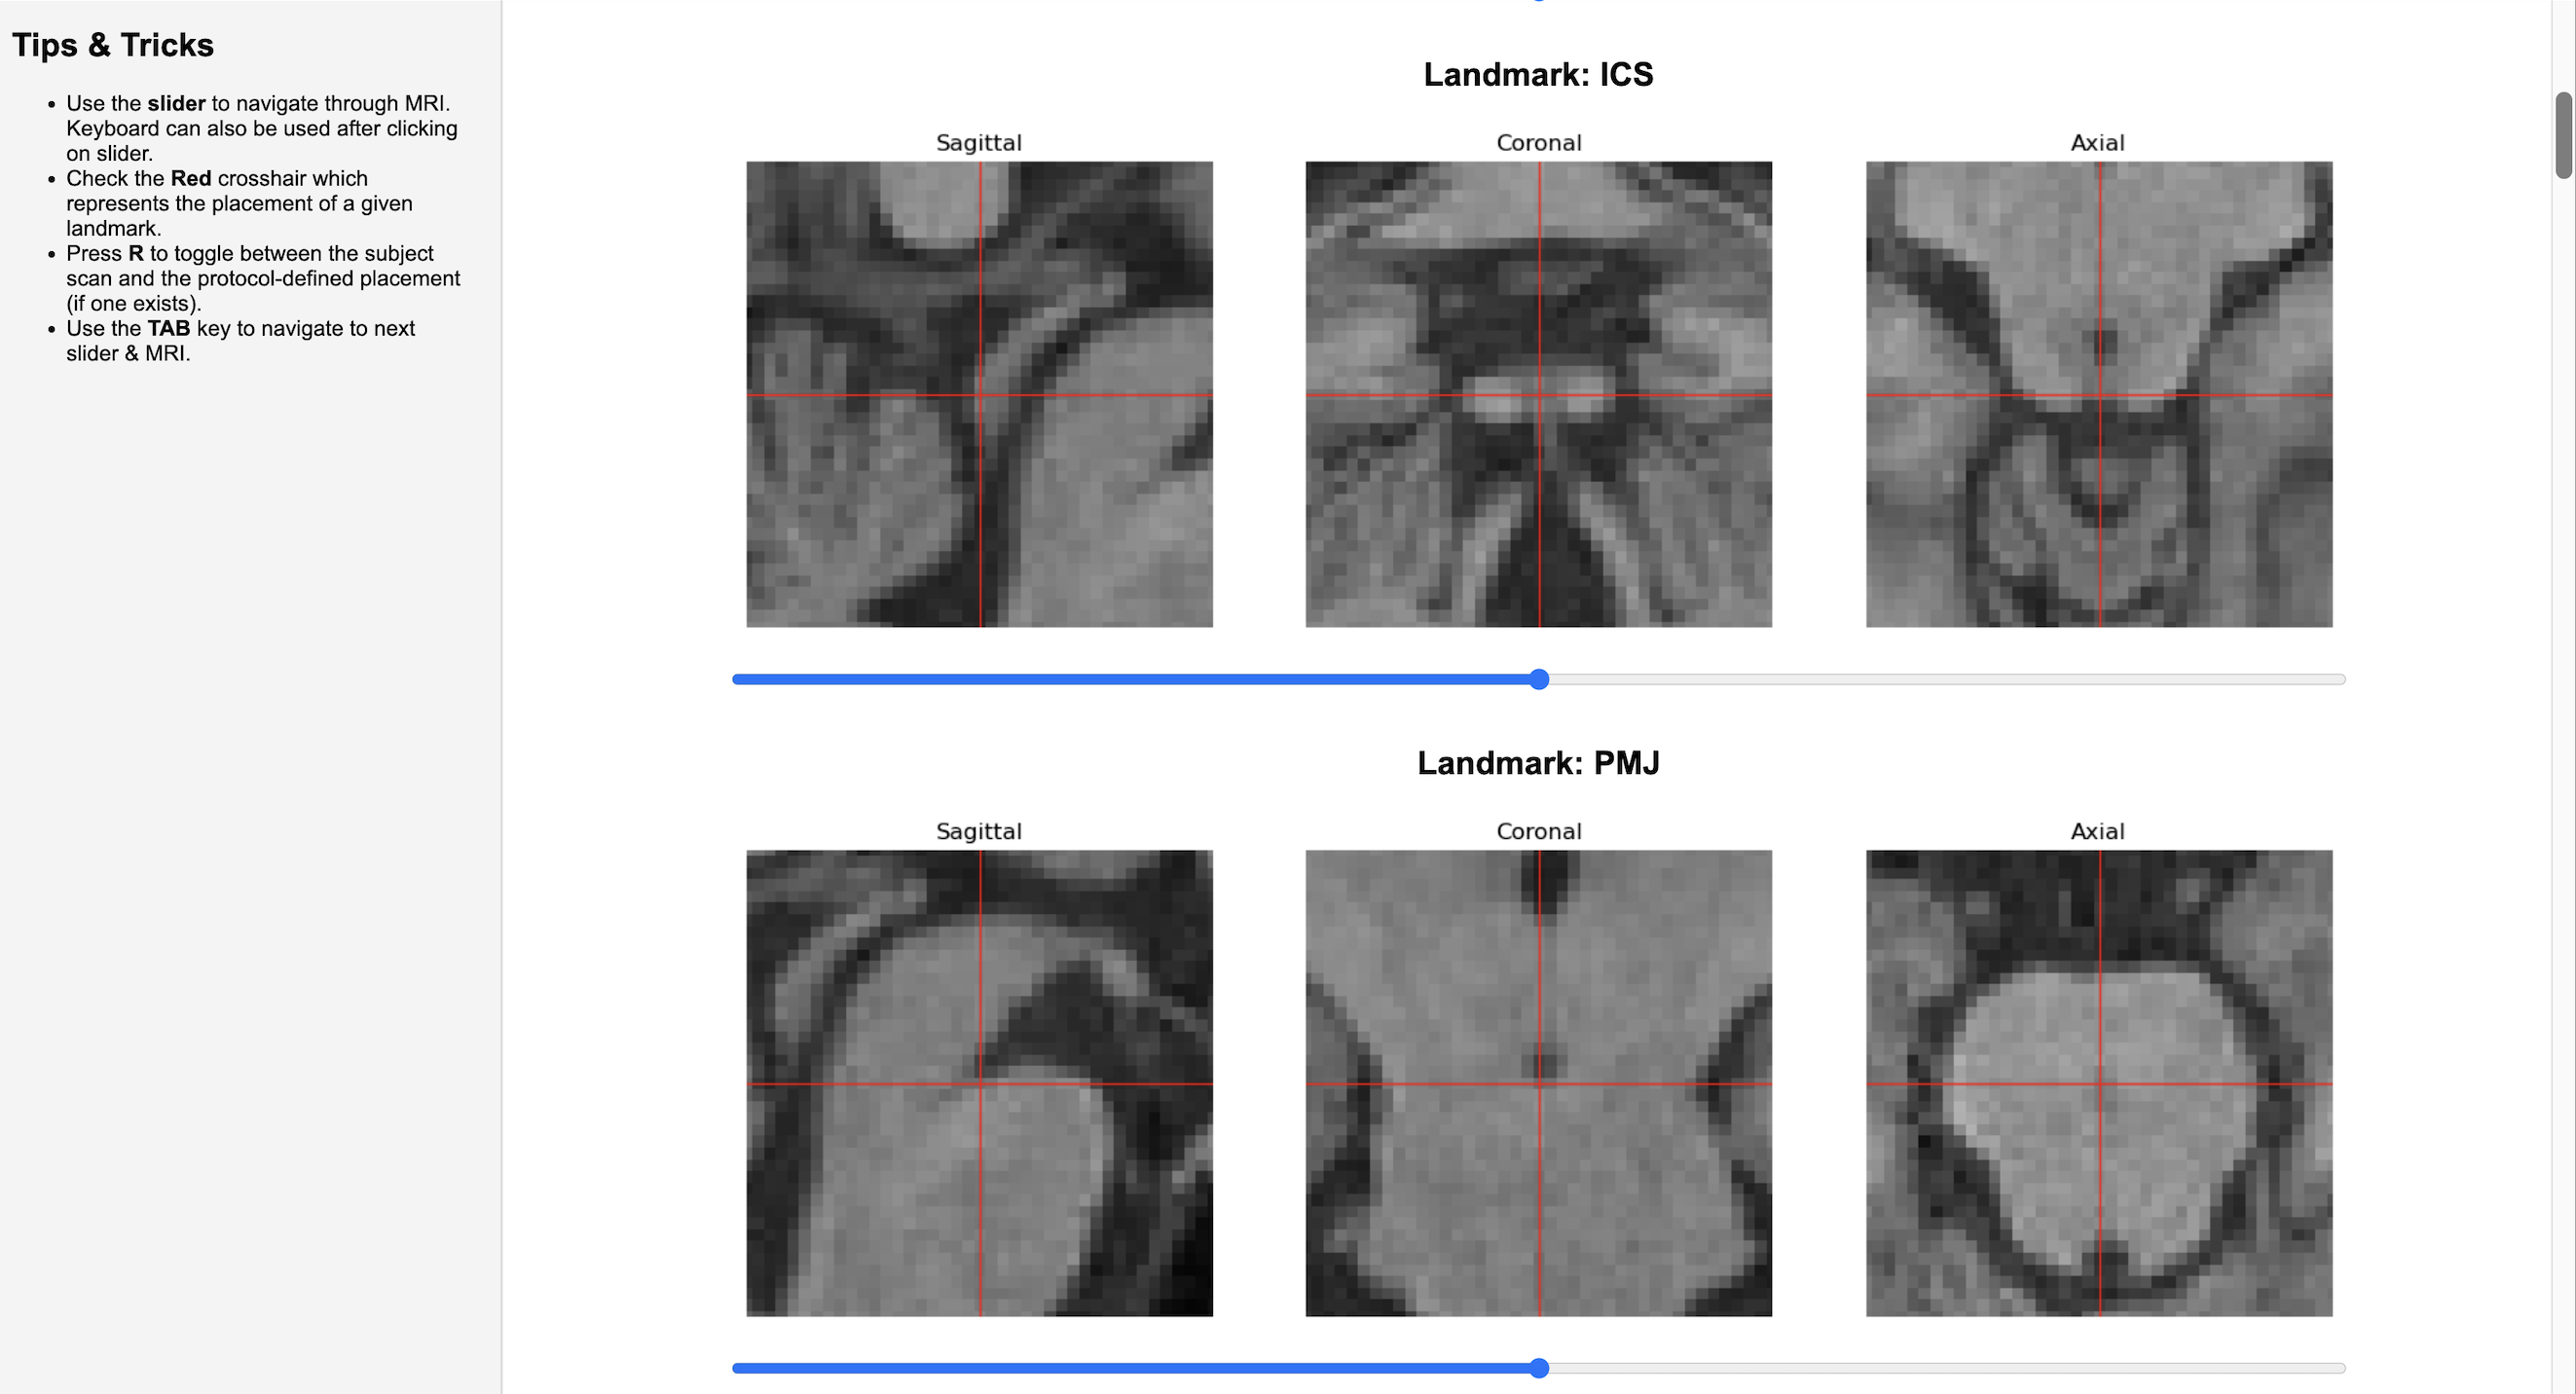
\includegraphics[width=1\linewidth]{figs/figuresupQC.png}
    \caption{Quality control visualization for anatomical landmark placement. Crosshairs indicate the annotated location of an example fiducial (the infracollicular sulcus [ICS]) in sagittal, coronal, and axial MRI views. Reviewers can toggle between the subject scan and the protocol-defined (template) annotation using the R key while navigating select slices in MRI volume using arrowkeys or slider.}
    \label{fig:figuresupQC}
\end{figure}

\newpage
\section{Hyperparameter Optimization}
Here we present the hyperparameter space used for both the ridge regressor and XGBoost. To prevent overfitting, we leveraged a custom \texttt{RepeatedGroupKFold} class to ensure that data splitting can be performed appropriately. 


\begin{minted}[fontsize=\small, bgcolor=bg, linenos, breaklines]{python}
# Ridge Regressor hyperparameters
alphas = np.logspace(-100, 100, 10000)  # Very wide range for RidgeCV tuning
k = 4                                   # Number of outer CV folds
var = 0.99                              # % variance to retain in PCA
\end{minted}

\begin{minted}[fontsize=\small, bgcolor=bg, linenos, breaklines]{python}
# XGBoost hyperparameters 
k = 4                                   # Number of outer CV folds
n_iter_search = 1000                    # Number of random search iterations
xgb_param_dist = dict(
    n_estimators= randint(50, 500),                 # boosting rounds
    max_depth= randint(2, 12),                      # model complexity
    learning_rate= uniform(0.01, 0.3),              # shrinkage
    subsample= uniform(0.6, 0.4),                   # row sampling
    colsample_bytree= uniform(0.6, 0.4),            # feature sampling
    gamma= uniform(0, 5),                           # min split loss
    reg_alpha= uniform(0, 1),                       # L1 regularization
    reg_lambda= uniform(0, 2)                       # L2 regularization
    )
\end{minted}

\begin{minted}[fontsize=\small, bgcolor=bg, linenos, breaklines]{python}
class RepeatedGroupKFold(_RepeatedSplits):
    """Repeated Group K-Fold cross validator.
    Repeats Group K-Fold n times with different randomization in each repetition.
    Parameters
    ----------
    n_splits : int, default=5
        Number of folds. Must be at least 2.
    n_repeats : int, default=10
        Number of times cross-validator needs to be repeated.
    random_state : int, RandomState instance or None, default=None
        Controls the randomness of each repeated cross-validation instance.
        Pass an int for reproducible output across multiple function calls.
        See :term:`Glossary <random_state>`.
    """
    def __init__(self, *, n_splits=5, n_repeats=10, random_state=None):
        super().__init__(
            GroupKFold, n_repeats=n_repeats,
            random_state=random_state, n_splits=n_splits)
        
    def split(self, X, y=None, groups=None):
        """Generates indices to split data into training and test set.
        Parameters
        ----------
        X : array-like of shape (n_samples, n_features)
            Training data, where n_samples is the number of samples
            and n_features is the number of features.
        y : array-like of shape (n_samples,)
            The target variable for supervised learning problems.
        groups : array-like of shape (n_samples,), default=None
            Group labels for the samples used while splitting the dataset into
            train/test set.
        Yields
        ------
        train : ndarray
            The training set indices for that split.
        test : ndarray
            The testing set indices for that split.
        """
        n_repeats = self.n_repeats
        rng = check_random_state(self.random_state)

        for idx in range(n_repeats):
            cv = self.cv(random_state=rng, shuffle=True,
                            **self.cvargs)
            for train_index, test_index in cv.split(X, y, groups):
                yield train_index, test_index
\end{minted}

\newpage
\section{Machine Learning Model Comparisons}\label{app:qualitycontrol}
We compared two machine learning models for coordinate-to-coordinate regression of the subthalamic nucelus (STN). Ridgre regression exhibited statistically lower errors in Euclidean error when compared to XGBoost. No significant difference was observed in the z-direction. Statistical comparisons were performed using Wilcoxon test (paired samples) with Bonferroni correction (\(\alpha = 0.05/4\))



\begin{figure}[hbt!]
    \centering
    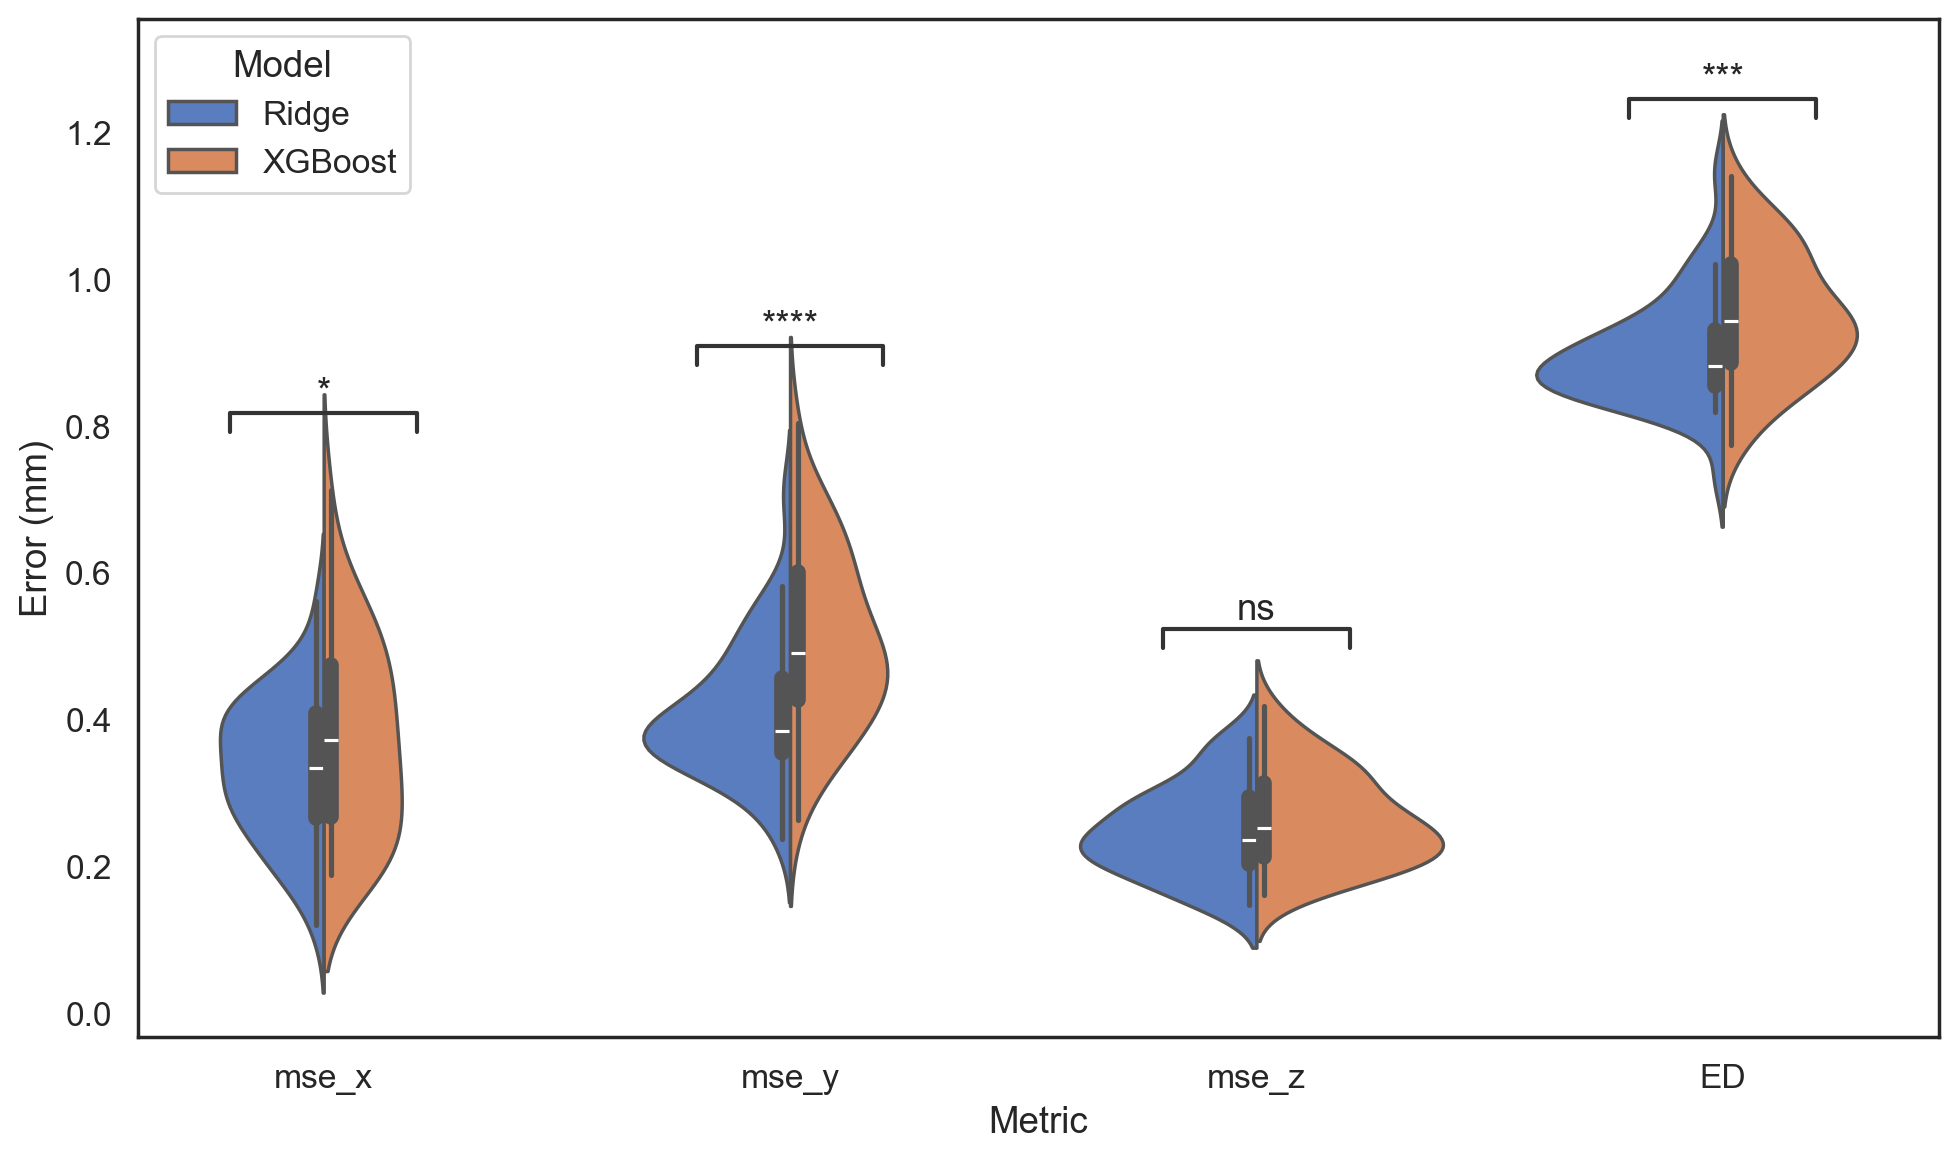
\includegraphics[width=1\linewidth]{figs/figuresupridgevsxgboost.png}
    \caption{Comparison of prediction errors between Ridge regression and XGBoost across spatial axes and Euclidean distance (ED). Violin plots show the distribution of per-fold prediction errors for each evaluation metric: mean squared error along the x, y, and z axes (\texttt{mse\_x}, \texttt{mse\_y}, \texttt{mse\_z}), and overall Euclidean distance (ED). Results are grouped by model type. Asterisks indicate the significance of paired comparisons between models using the Wilcoxon signed-rank test (\textit{p}\(<\)0.05: *, \textit{p}\(<\)0.01: **, \textit{p}\(<\)0.001: ***, \textit{p}\(<\)0.0001: ****; ns: not significant).}
    \label{fig:figuresupridgevsxgboost}
\end{figure}

\newpage
\section{AFIDs Stereotaxy Website}\label{app:stereotaxy}
We packaged our model and deployed it on a website (\url{https://stereotaxy.afids.io/}) along side the factored protocol of the 16 anatomical fiducials used to predict the subthalamic nucleus. Figure \ref{fig:figuresupstereotaxy} provides a snapshot of the website for completeness. 

\begin{figure}[hbt!]
    \centering
    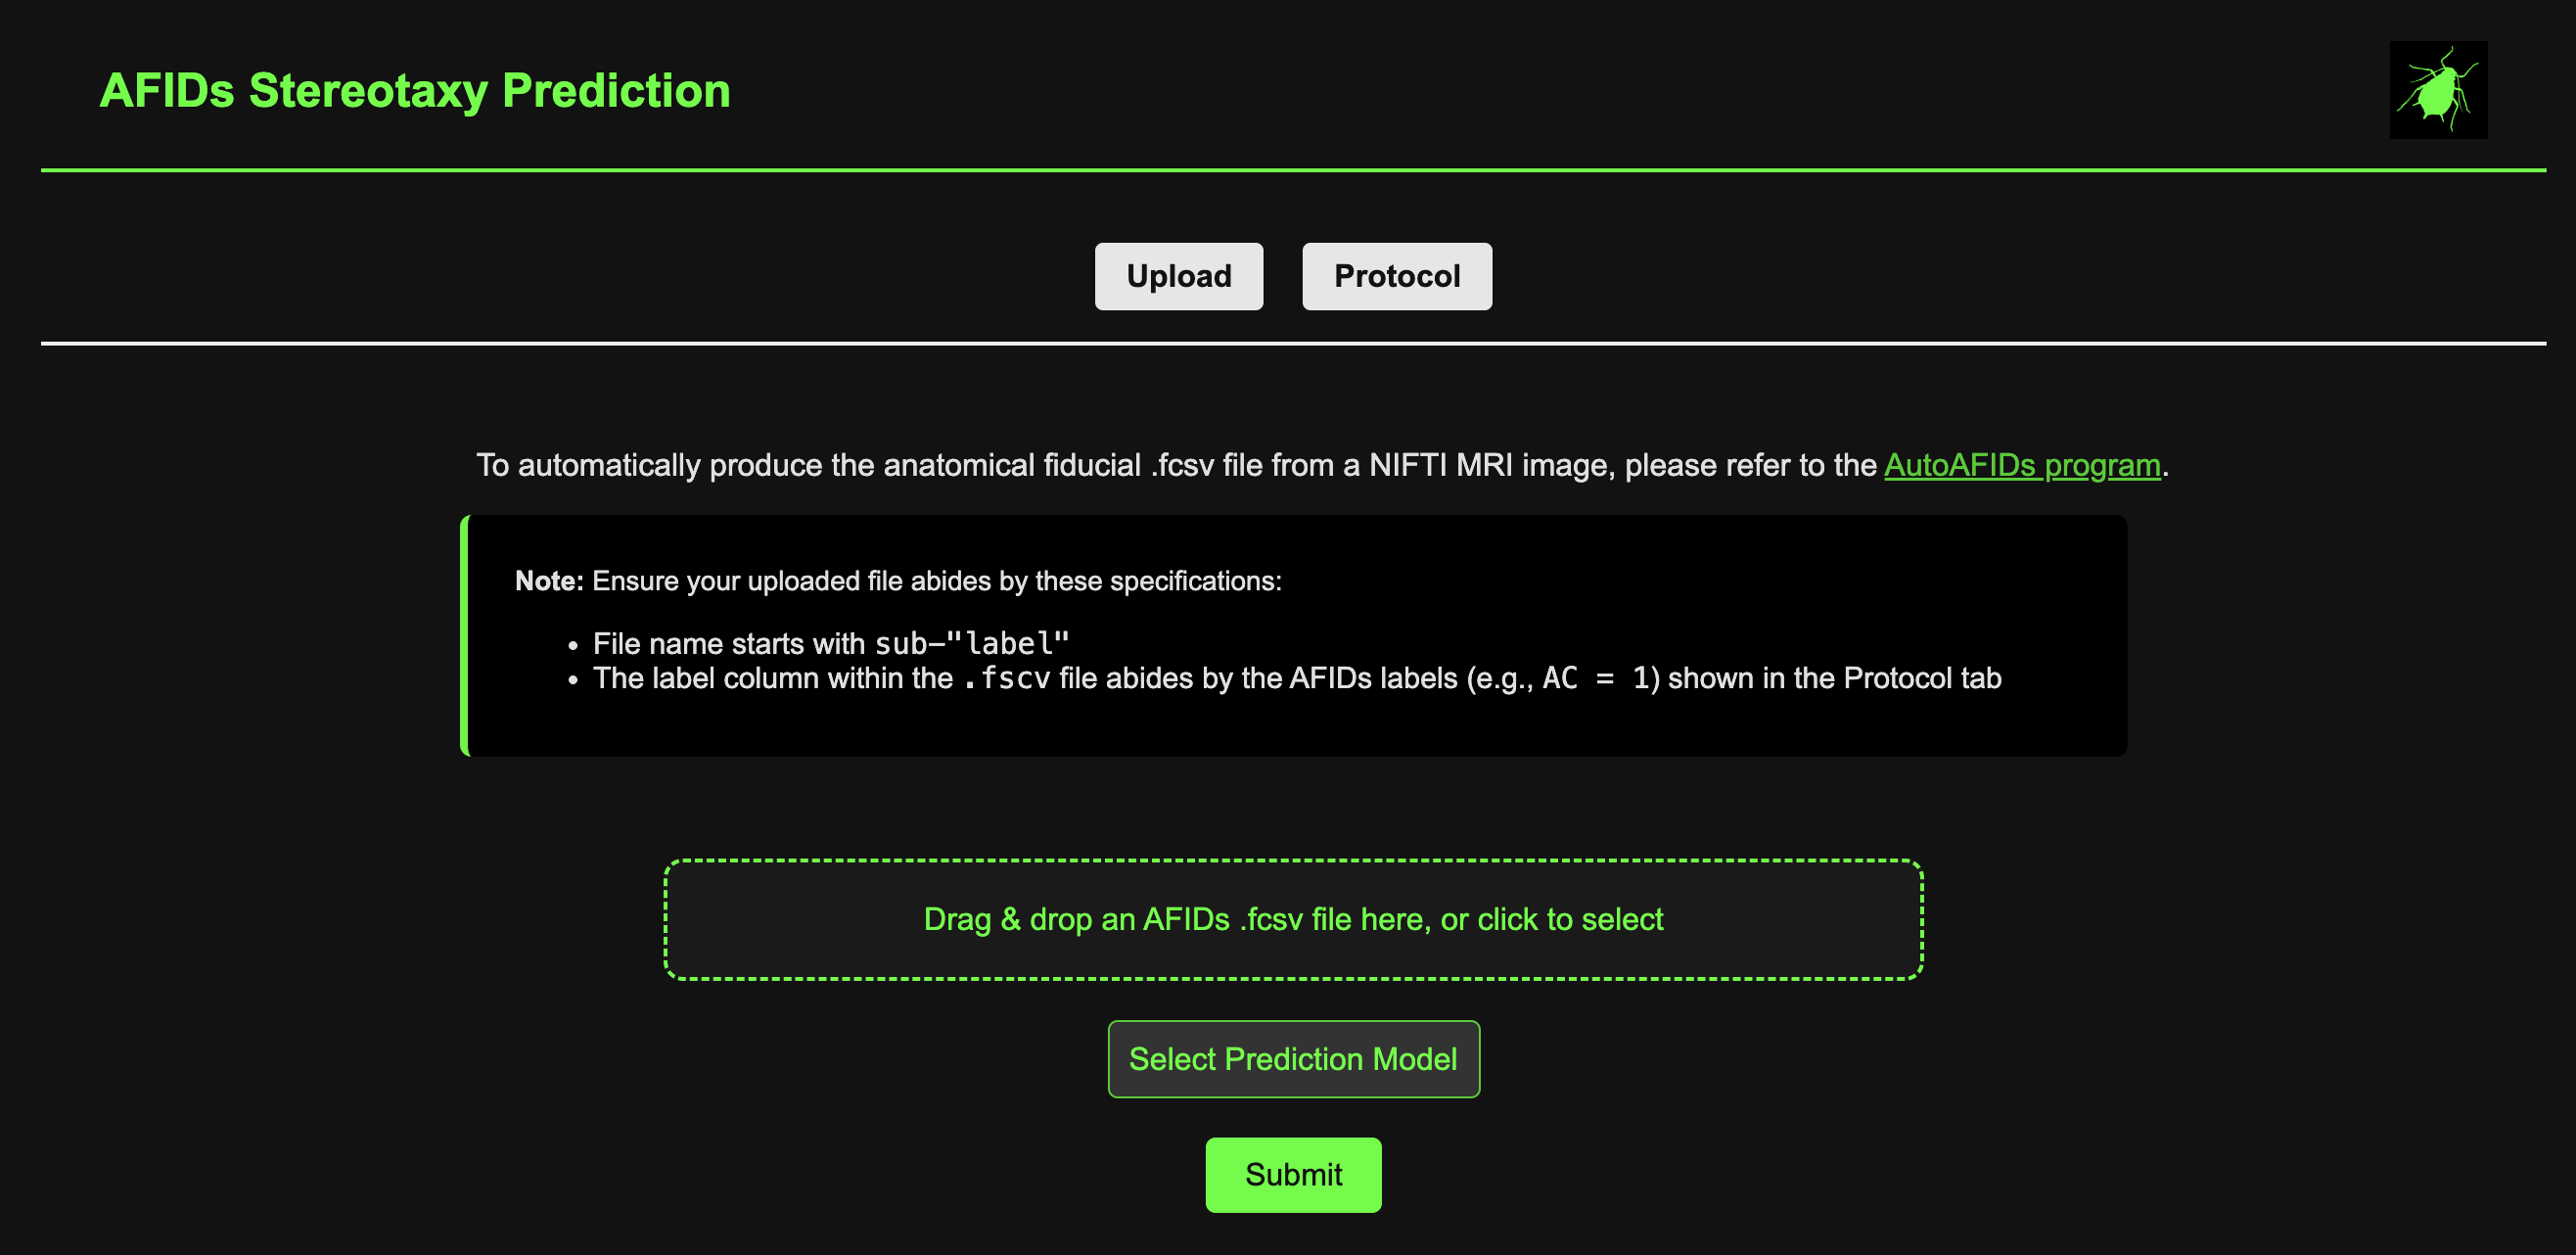
\includegraphics[width=1\linewidth]{figs/figuresupstereotaxy.png}
    \caption{Users can upload anatomical fiducial (AFID) annotations in \texttt{.fcsv} format, typically generated using 3D Slicer. Currently, the platform supports target prediction for the subthalamic nucleus (STN), with plans to expand support to additional structures such as the caudal zona incerta and various thalamic subnuclei. Upon submission, the selected model runs on the backend and returns predicted target coordinates in both native and AC--PC space. The platform also includes a protocol panel displaying the reduced protocol, currently consisting of 16 AFIDs.}
    \label{fig:figuresupstereotaxy}
\end{figure}
